% ------------------------------------------------------------------------------
% TYPO3 CMS 7.4 - What's New - Chapter "Introduction" (English Version)
%
% @author	Michael Schams <schams.net>
% @license	Creative Commons BY-NC-SA 3.0
% @link		http://typo3.org/download/release-notes/whats-new/
% @language	English
% ------------------------------------------------------------------------------
% LTXE-CHAPTER-UID:		9dc37b9a-9fad14c3-bf7eabfd-82b83622
% LTXE-CHAPTER-NAME:	Introduction
% ------------------------------------------------------------------------------

\section{Introducción}
\begin{frame}[fragile]
	\frametitle{Introducción}

	\begin{center}\huge{Introducción}\end{center}
	\begin{center}\huge{\color{typo3darkgrey}\textbf{Los Hechos}}\end{center}

\end{frame}

% ------------------------------------------------------------------------------
% LTXE-SLIDE-START
% LTXE-SLIDE-UID:		14e7179a-52e83a2e-b770d3f8-440dd85c
% LTXE-SLIDE-ORIGIN:	3cc566cf-d7166203-45a36415-7c8e8ebf English
% LTXE-SLIDE-ORIGIN:	5d8622ac-37911548-171bf8ec-5add4ed5 German
% LTXE-SLIDE-TITLE:		TYPO3 CMS 7.4 - The Facts
% ------------------------------------------------------------------------------
\begin{frame}[fragile]
	\frametitle{Introducción}
	\framesubtitle{TYPO3 CMS 7.4 - Los Hechos}

	\begin{itemize}
		\item Fecha de lanzamiento: 04. Agosto 2015
		\item Tipo de lanzamiento: "Lanzamiento Sprint"
		\item Visión: Adoptar, Innovar, Lanzar
		\item Foco principal: Revisión de Backend Vol 2
	\end{itemize}

\end{frame}

% ------------------------------------------------------------------------------
% LTXE-SLIDE-START
% LTXE-SLIDE-UID:		a9f6dd5e-84692bce-c520ff68-e173d9db
% LTXE-SLIDE-ORIGIN:	6746e3bc-a8575d0c-e1681766-d0d78911 English
% LTXE-SLIDE-ORIGIN:	9da27f39-55d99c31-9ee9136a-20d96c0e German
% LTXE-SLIDE-TITLE:		System Requirements
% ------------------------------------------------------------------------------
\begin{frame}[fragile]
	\frametitle{Introducción}
	\framesubtitle{Requisitos del Sistema}

	\begin{itemize}
		\item PHP*:\tabto{2.2cm}v5.5.0 - v5.6.x
		\item MySQL:\tabto{2.2cm}v5.5.x - v5.6.x (modo no estricto)
		\item Espacio de disco:\tabto{3.4cm}mín 200 MB
		\item Ajustes de PHP:

			\begin{itemize}
				\item memory\_limit >= 128M
				\item max\_execution\_time >= 240s
				\item opción de compilación \texttt{--disable-ipv6} \underline{no} debe ser usada
			\end{itemize}

		\item Backend requiere IE >= 9 o cualquier otro navegador moderno

	\end{itemize}

	\vspace{1cm}
	*) Detalles adicionales: \href{http://typo3.org/news/article/php-minimum-requirements-for-typo3-cms-7/}{Requisitos Mínimos de PHP para TYPO3 CMS 7}

\end{frame}

% ------------------------------------------------------------------------------
% LTXE-SLIDE-START
% LTXE-SLIDE-UID:		9eb9a29c-9bfdcb73-57c28beb-f051f7d1
% LTXE-SLIDE-ORIGIN:	081f8b1d-b8f58841-dccf8d1d-148fd25d English
% LTXE-SLIDE-ORIGIN:	dbbfebbe-fb43ddb8-bca9ae69-716b8a0f German
% LTXE-SLIDE-TITLE:		Development And Release Timeline
% ------------------------------------------------------------------------------
\begin{frame}[fragile]
	\frametitle{Introducción}
	\framesubtitle{Línea de tiempo de Desarrollo y Lanzamiento}

	\begin{figure}
		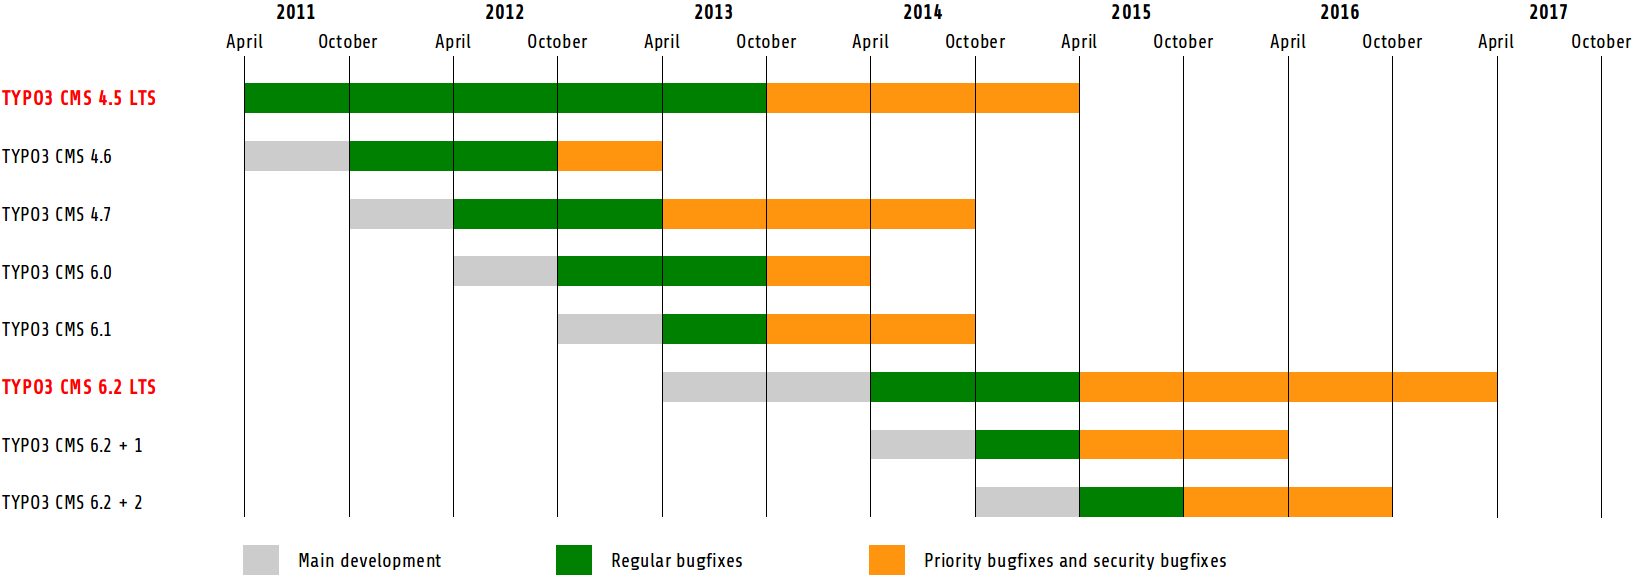
\includegraphics[width=0.90\linewidth]{Introduction/ReleaseAgenda.png}
	\end{figure}

\end{frame}

% ------------------------------------------------------------------------------
% LTXE-SLIDE-START
% LTXE-SLIDE-UID:		274ba9c4-ba6d55b2-5edd53af-a000ab7f
% LTXE-SLIDE-ORIGIN:	a5555bb0-f1f8031f-f271766a-2dbc1b08 English
% LTXE-SLIDE-ORIGIN:	e359142e-e7c10774-5d851da9-b26a275b German
% LTXE-SLIDE-TITLE:		TYPO3 CMS Roadmap
% ------------------------------------------------------------------------------
\begin{frame}[fragile]
	\frametitle{Introducción}
	\framesubtitle{Línea de lanzamiento de TYPO3 CMS}

	Fechas de lanzamiento estimadas y sus enfoques principales:

	\begin{itemize}
		\item v7.0 \tabto{1.0cm}02/Dic/2014\tabto{3.4cm}Revisión de Backend Vol 1
		\item v7.1 \tabto{1.0cm}24/Feb/2015\tabto{3.4cm}Optimización \& Limpieza del núcleo
		\item v7.2 \tabto{1.0cm}28/Apr/2015\tabto{3.4cm}Frontend
		\item v7.3 \tabto{1.0cm}16/Jun/2015\tabto{3.4cm}Ecosistema de Paquetes, Composer\newline
			\tabto{3.4cm}y Manejo de Extensiones
		\item
			\begingroup
				\color{typo3orange}
					v7.4 \tabto{1.0cm}04/Ago/2015\tabto{3.4cm}Revisión de Backend Vol 2
			\endgroup

		\item v7.5 \tabto{1.0cm}29/Sep/2015\tabto{3.4cm}\textit{(por determinar...)}
		\item v7.6 \tabto{1.0cm}xx/xxx/2015\tabto{3.4cm}\textbf{TYPO3 CMS 7 LTS} (Long Term Release)
	\end{itemize}

	\smaller
		\url{https://typo3.org/typo3-cms/roadmap/}\newline
		\url{http://typo3.org/news/article/embrace-and-innovate-typo3-cms-7/}
	\normalsize

\end{frame}

% ------------------------------------------------------------------------------
% LTXE-SLIDE-START
% LTXE-SLIDE-UID:		6b085ccd-53e0329b-b26695b2-891e8f54
% LTXE-SLIDE-ORIGIN:	5ef3ad6d-b72464d3-6a2867a6-298cb382 English
% LTXE-SLIDE-ORIGIN:	c8966352-3e5159b9-f0e3ea35-9d4455ef German
% LTXE-SLIDE-TITLE:		Installation
% ------------------------------------------------------------------------------
\begin{frame}[fragile]
	\frametitle{Introducción}
	\framesubtitle{Instalación}

	\begin{itemize}
		\item Procedimiento de instalación oficial bajo Linux/Mac OS X\newline
			(DocumentRoot por ejemplo \texttt{/var/www/site/htdocs}):
		\begin{lstlisting}
			$ cd /var/www/site
			$ wget --content-disposition get.typo3.org/7.4
			$ tar xzf typo3_src-7.4.0.tar.gz
			$ cd htdocs
			$ ln -s ../typo3_src-7.4.0 typo3_src
			$ ln -s typo3_src/index.php
			$ ln -s typo3_src/typo3
			$ touch FIRST_INSTALL
		\end{lstlisting}

		\item Enlaces simbólicos bajo Microsoft Windows:

			\begin{itemize}
				\item Use \texttt{junction} en Windows XP/2000
				\item Use \texttt{mlink} en Windows Vista y Windows 7
			\end{itemize}

	\end{itemize}
\end{frame}

% ------------------------------------------------------------------------------
% LTXE-SLIDE-START
% LTXE-SLIDE-UID:		2975909e-dccef957-5d504c82-690bef13
% LTXE-SLIDE-ORIGIN:	12551741-9cb07199-fb3614d0-1a242a5f English
% LTXE-SLIDE-ORIGIN:	af099855-2b970b2b-89ed7d02-7219b2b9 German
% LTXE-SLIDE-TITLE:		Upgrade to TYPO3 CMS 7
% ------------------------------------------------------------------------------
\begin{frame}[fragile]
	\frametitle{Introducción}
	\framesubtitle{Actualización a TYPO3 CMS 7.x}

	\begin{itemize}
		\item Actualizaciones sólo posibles desde TYPO3 CMS 6.2 LTS
		\item TYPO3 CMS < 6.2 debe ser actualizado a TYPO3 CMS 6.2 LTS primero
	\end{itemize}

	\begin{itemize}

		\item Instrucciones de actualización:\newline
			\smaller\url{http://wiki.typo3.org/Upgrade#Upgrading_to_7.4}\normalsize
		\item Guía oficial de TYPO3 "Instalación y Actualización de TYPO3":
			\smaller\url{http://docs.typo3.org/typo3cms/InstallationGuide}\normalsize
		\item Enfoque general:
			\begin{itemize}
				\item Comprobar requisitos mínimos del sistema \small(PHP, MySQL, etc.)
				\item Revisar \textbf{deprecation\_*.log} en instancia antigua de TYPO3
				\item Actualizar todas las extensiones a la última versión
				\item Desplegar fuentes nuevas y ejecutar Herramienta de Instalación \textrightarrow Asistente de Actualización
				\item Revisar el módulo de inicio para usuarios backend (opcionalmente)
			\end{itemize}
	\end{itemize}

\end{frame}

% ------------------------------------------------------------------------------
